\documentclass{article}
\usepackage{hyperref}
\usepackage{float}
\usepackage{graphicx}

\begin{document}

\title{Business Ethics of Autonomous Cars}
\author{Kevin Schoonover}

\maketitle

\begin{abstract}
Americans spend on average 308 hours driving~\cite{aaa} and cause on average
35,000 fatalities~\cite{nhtsa_fatalities} every year. The advent of autonomous
cars allow drivers to reclaim these 308 hours while saving over 35,000 lives
if implemented perfectly. However, theoretical possibility proved to be far
from reality when autonomous vehicles had fatal crashes from
Uber~\cite{uber} and Tesla~\cite{tesla}. These crashes beg the questions: `How
good must an autonomous car be before an company should release it?' and `Who
is at fault -- the company, the driver, or the other person?'
\end{abstract}

\section{Project}
The project will explore potential answers to the questions by building a web
application that will guide subjects through a series of scenarios and store
their response. Then, all results will be condensed and examined in a 1-2 page
final report, not including the data tables.

\subsection{Scenarios}
The \textbf{first scenario} will test the subject on three different stories
regarding autonomous vehicle crashes. The subject will read a story, select who
they think is at fault (the company, the driver, or the other person), and move
onto the next story. They must choose only one they believe is most at fault.
The stories will be as follows:
\begin{enumerate}
  \item Present the story of the Uber crash presented in~\cite{uber}, but
    anonymize the names and locations to prevent the subject from easily
    recognizing the story.
  \item Present the story of the Tesla crash presented in~\cite{tesla} following
    the same anonymization strategy.
  \item Present a story created by the researcher. This story will contain
    dialog that puts all three potential options into question. An example
    abstract for a story: The company developed a perfect autonomous car;
    however, when it is snowy outside a design flaw makes the car unable to
    detect distant items. The driver fell asleep while traveling to see their
    parents on Christmas (and it was snowing) and signed a licenses agreement
    that the car may not work perfectly in all circumstances. A pedestrian, who
    also cannot see because of the snow, crosses the street and is killed.
\end{enumerate}

The subject will be asked after each question to explain their reasoning of why
they believe each particular person/company is at fault. When the final story is
complete, the user will move on to scenario two.

The \textbf{second scenario} will determine how well an autonomous vehicle needs
to operate before the user will buy it. A series of 5 statements will be
presented that the user will rate from 1 (Highly disagree) to 5 (Strongly
Agree). The statements are as follows:
\begin{itemize}
  \item Autonomous mode must be able to operate in vision impairing rain and/or
    snow.
  \item Autonomous mode must be able to operate during non vision impairing rain
    and/or snow.
  \item Autonomous mode must be able to operate on a sunny day.
  \item Autonomous mode must be able to operate during the night.
  \item Autonomous mode must work while I am asleep or performing another action.
  \item Autonomous mode must function better than a human.
\end{itemize}

These questions will be asked twice prefaced with two different modes of
autonomous driving (fully autonomous and conditional autonomous)\footnote{See
\url{https://cyberlaw.stanford.edu/blog/2013/12/sae-levels-driving-automation}
for more information}. Each definition will be explained before the questions to
give the subject background information.

\subsection{Web Application}
The web application will have two screens for the different scenarios:
\begin{figure}[H]
\centering
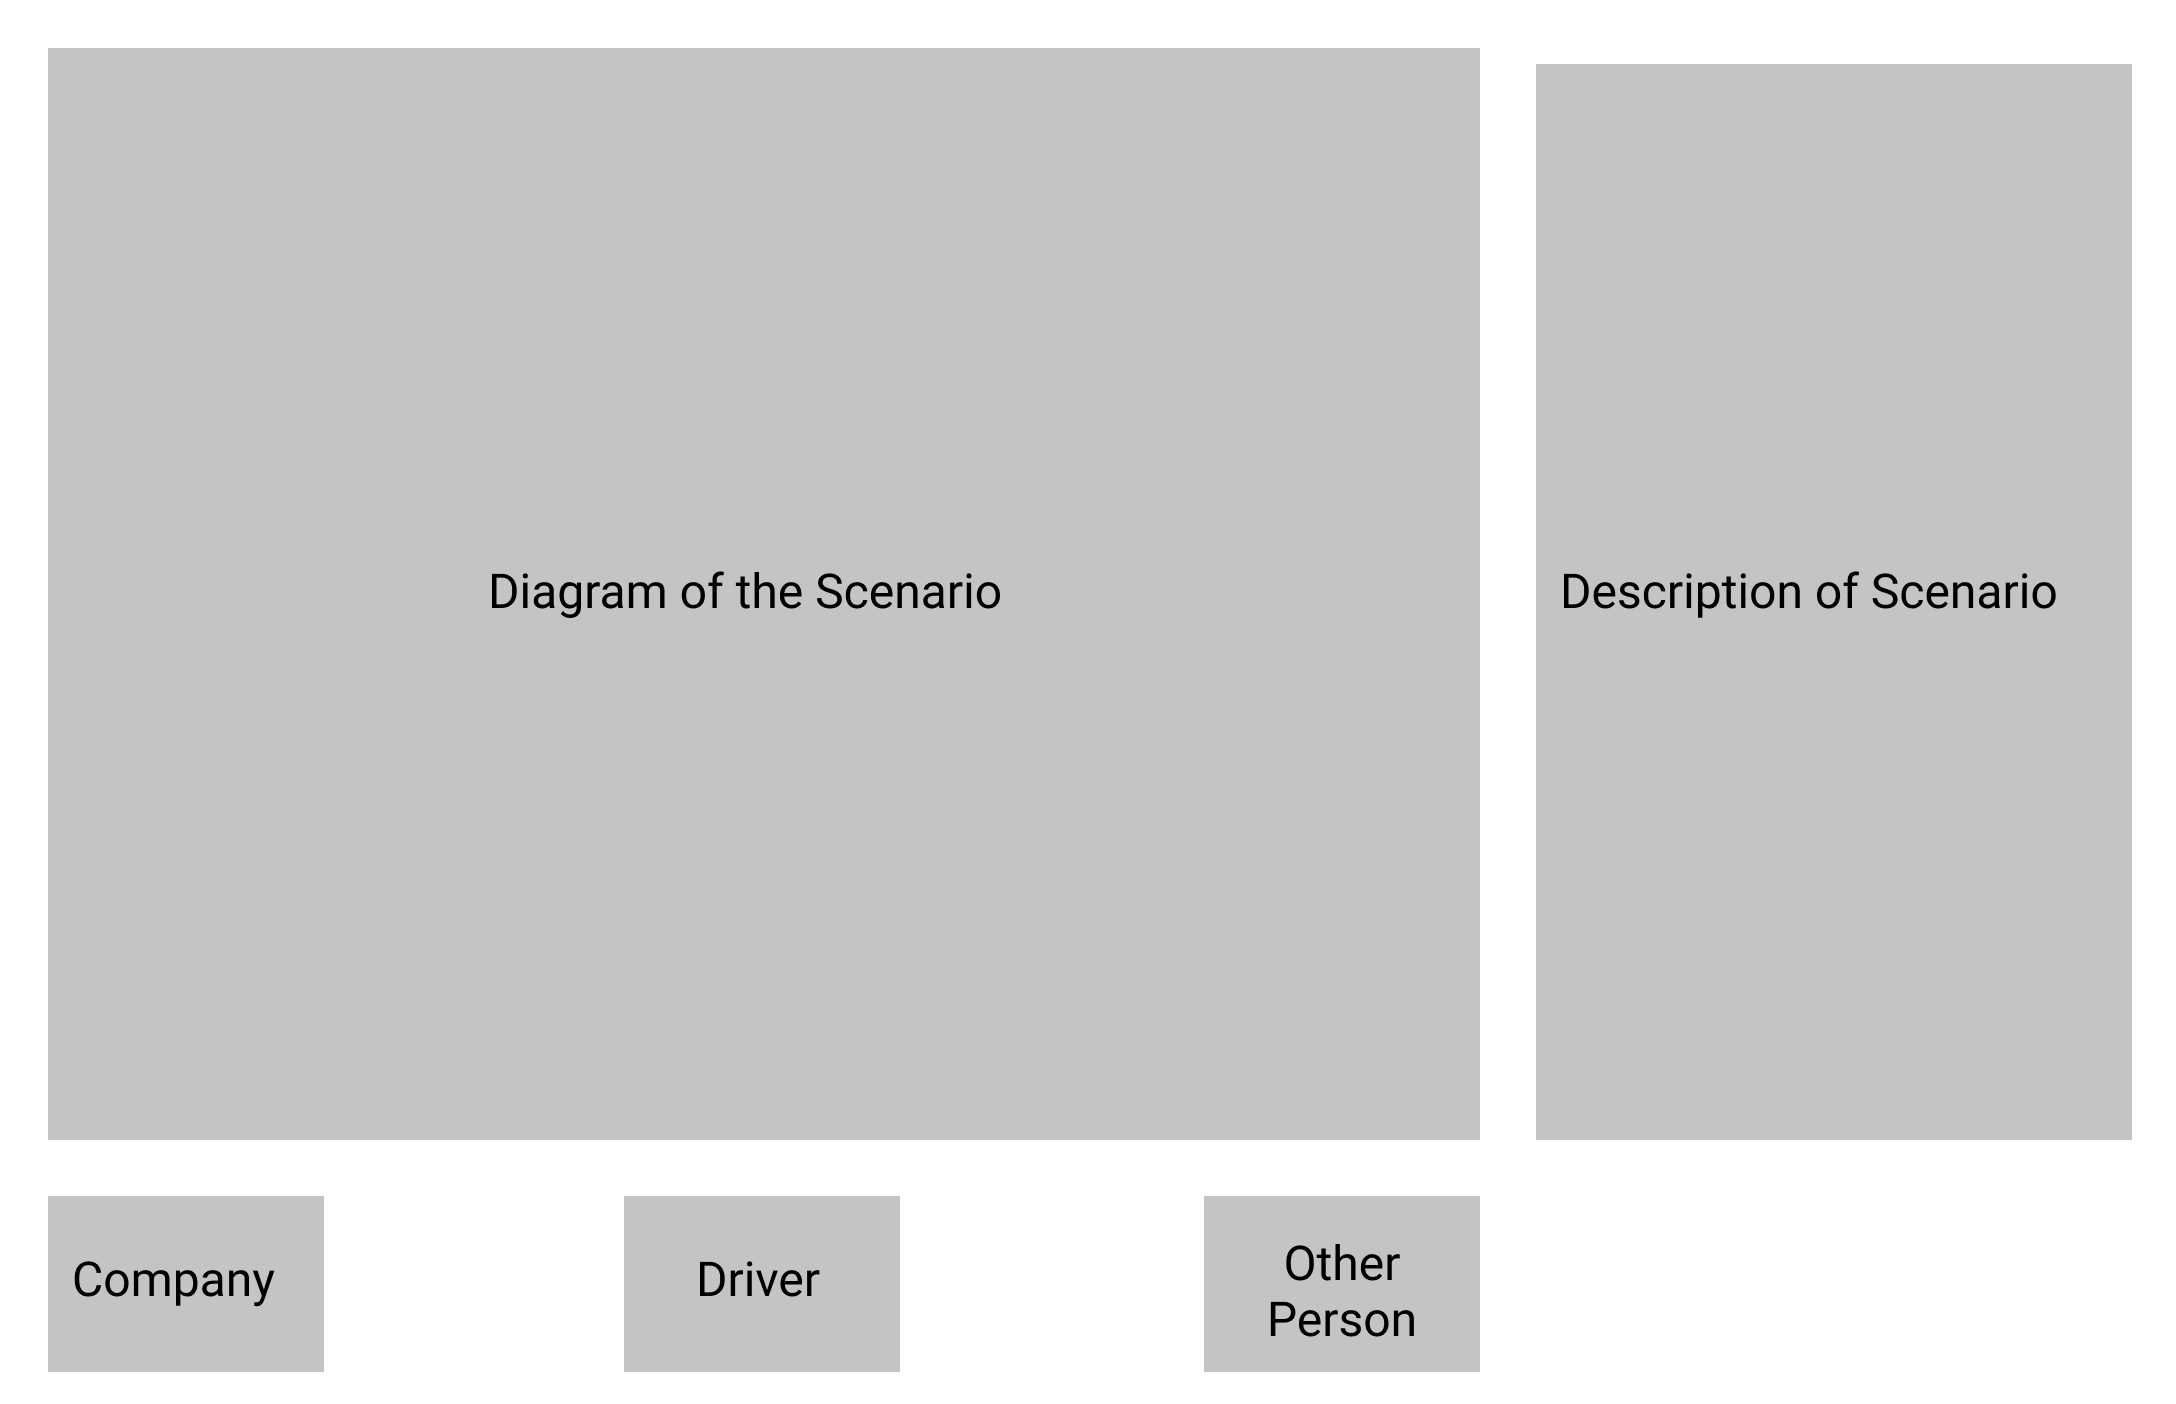
\includegraphics[height=2.5in]{imgs/scenario_1.png}
\caption{Scenario 1 Mock up}
\label{fig:scenario_1}
\end{figure}

Figure \ref{fig:scenario_1} shows abstractly how the page for scenario 1 will
look.

\begin{figure}[H]
\centering
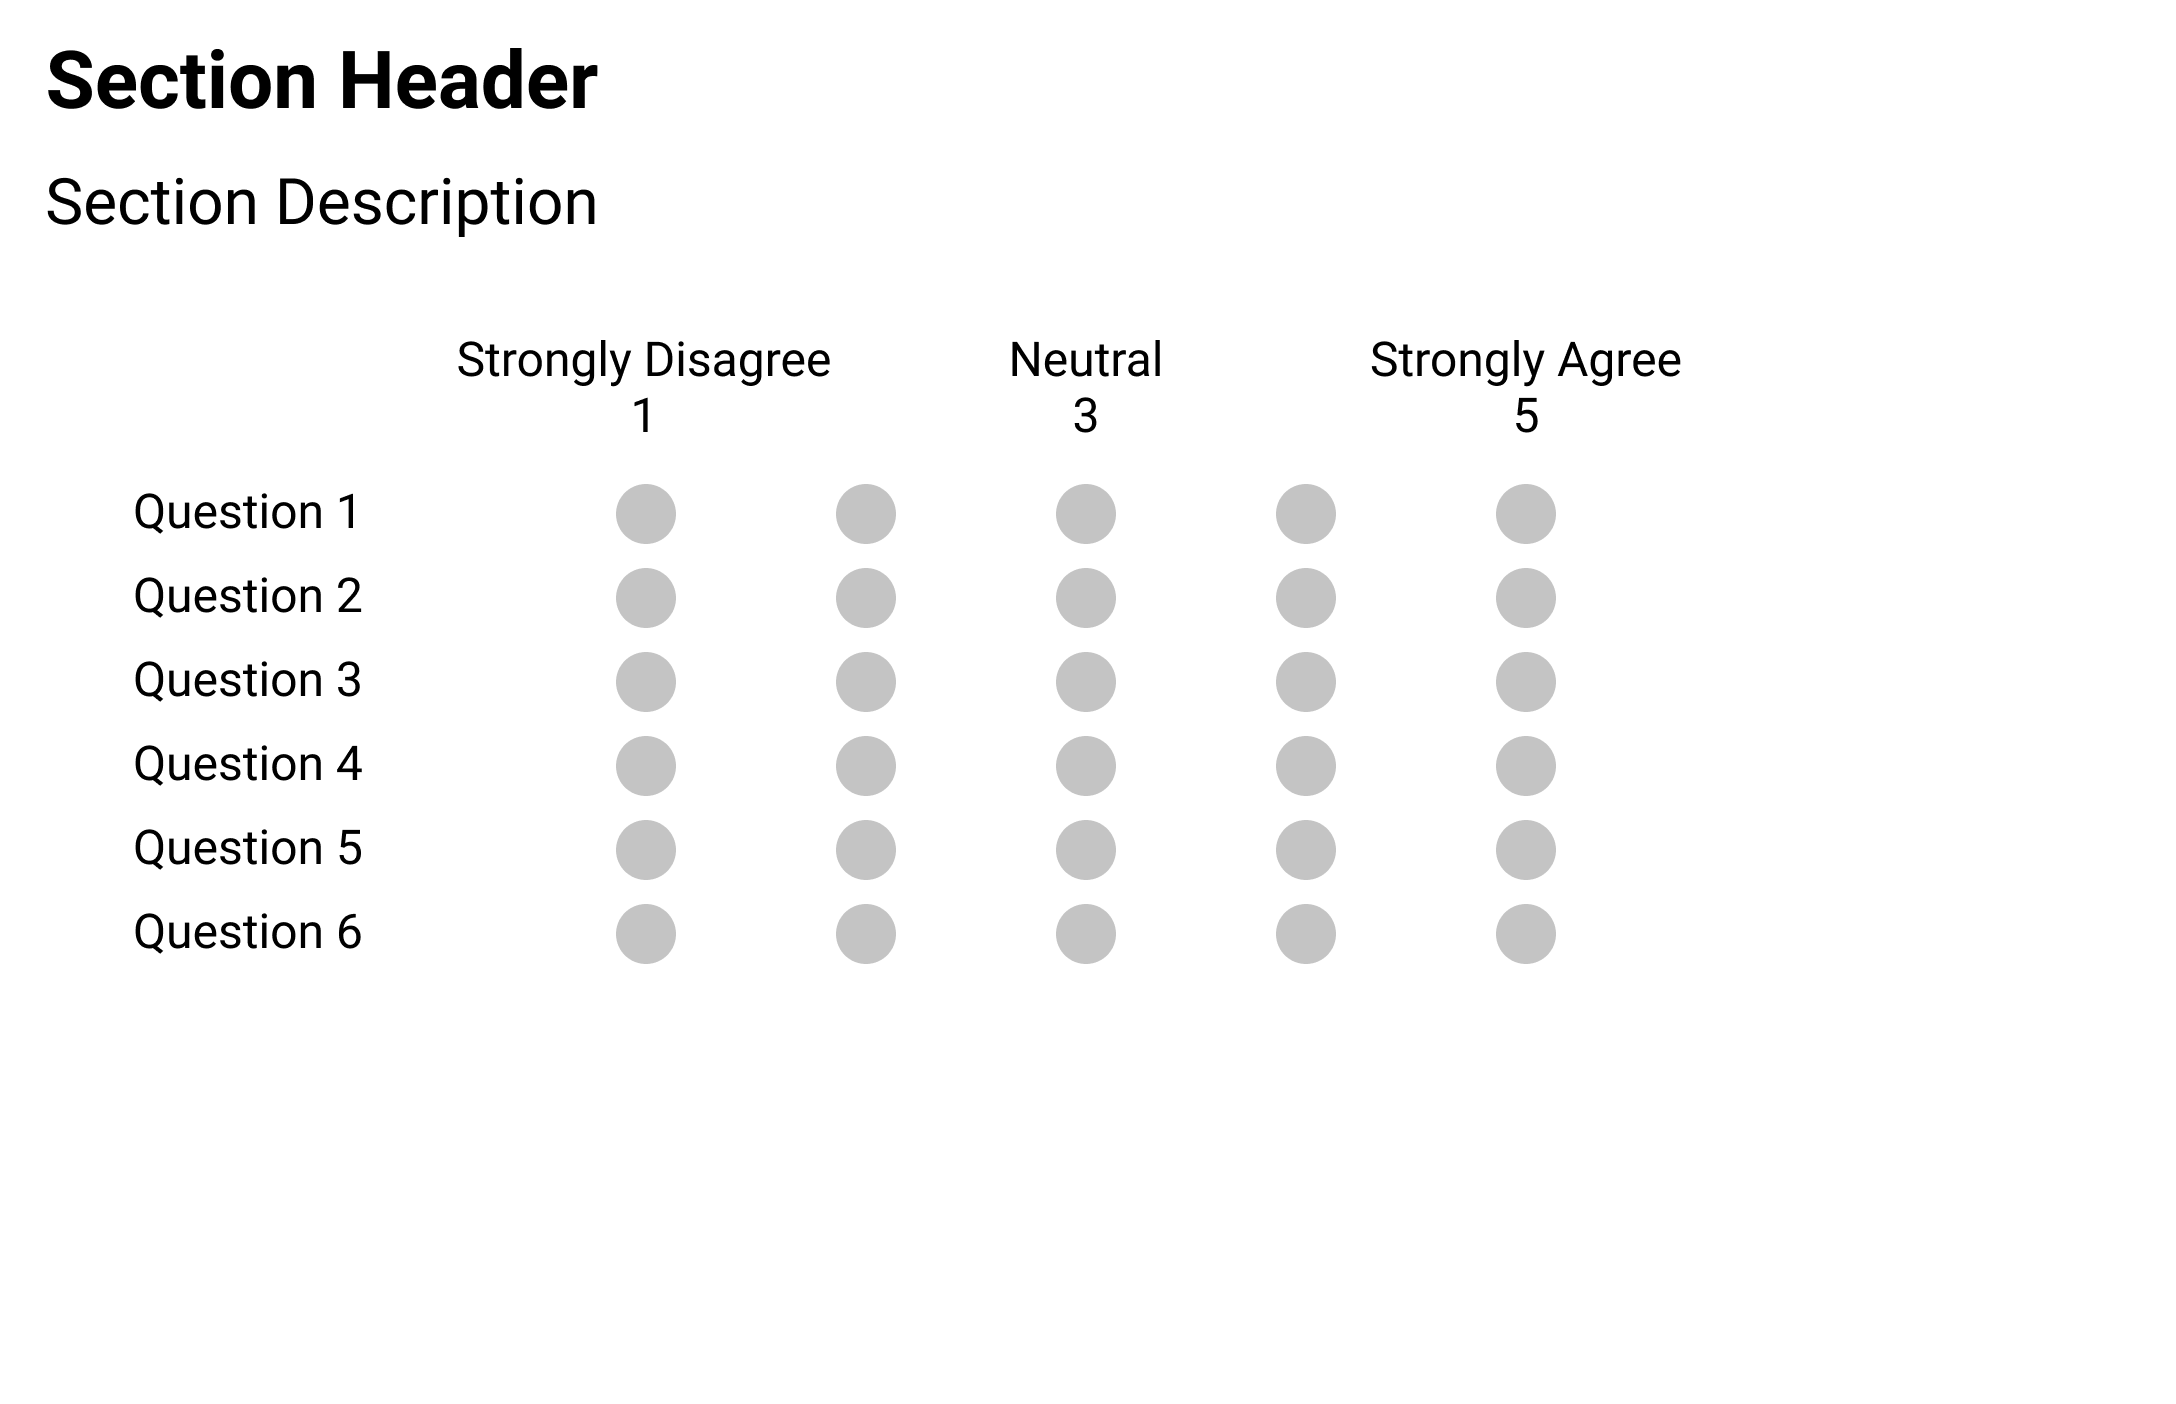
\includegraphics[height=3in]{imgs/scenario_2.png}
\caption{Scenario 2 Mock up}
\label{fig:scenario_2}
\end{figure}

Figure \ref{fig:scenario_2} shows abstractly how the page for scenario 2 will
look.

\subsection{Final Report}
After results are collected from 5-10 subjects, I will synthesize a final report
summarizing the conclusions. The 1-2 page analysis will focus on if there was a
general consensus among the participants, display graphics with the overall
results, distill why participants responded certain ways, and propose an answer
to the original questions.

\section{Rubric}
\begin{itemize}
  \item \textbf{Scenarios} (20 points)
  \begin{itemize}
    \item Design of custom autonomous car story (5/20 points)
    \item Presentation of Uber and Tesla stories (5/20 points)
    \item Gathering and recording of results (10/20 points)
  \end{itemize}

  \item \textbf{Web Application} (20 points)
  \begin{itemize}
    \item Functionality of pages (10/20 points)
    \item Design of pages (5/20 points)
    \item Persistent storage and visualization of results (5/20 points)
  \end{itemize}

  \item \textbf{Final Report} (20 points)
  \begin{itemize}
    \item Grammar, spelling, and punctuation (5/20 points)
    \item Conclusions from the results (15/20 points)
  \end{itemize}

\end{itemize}

\bibliographystyle{plain}
\bibliography{bib/references}

\end{document}
